\item A bobina tem massa de \SI{75}{\kilogram} e raio de giração $k_{O}=\SI{.675}{\meter}$. Se uma corda é enrolada em torno de seu miolo interno e sua extremidade é puxada com uma força horizontal $P=\SI{200}{\newton}$, determine a velocidade angular da bobina após o centro $O$ ter se movido $\SI{3}{\meter}$ para a direita. A bobina parte do repouso e não desliza em $A$ enquanto rola. Despreze a massa da corda.

\import{../answers}{answer-5}

\vspace{-1cm}
\begin{flushright}
	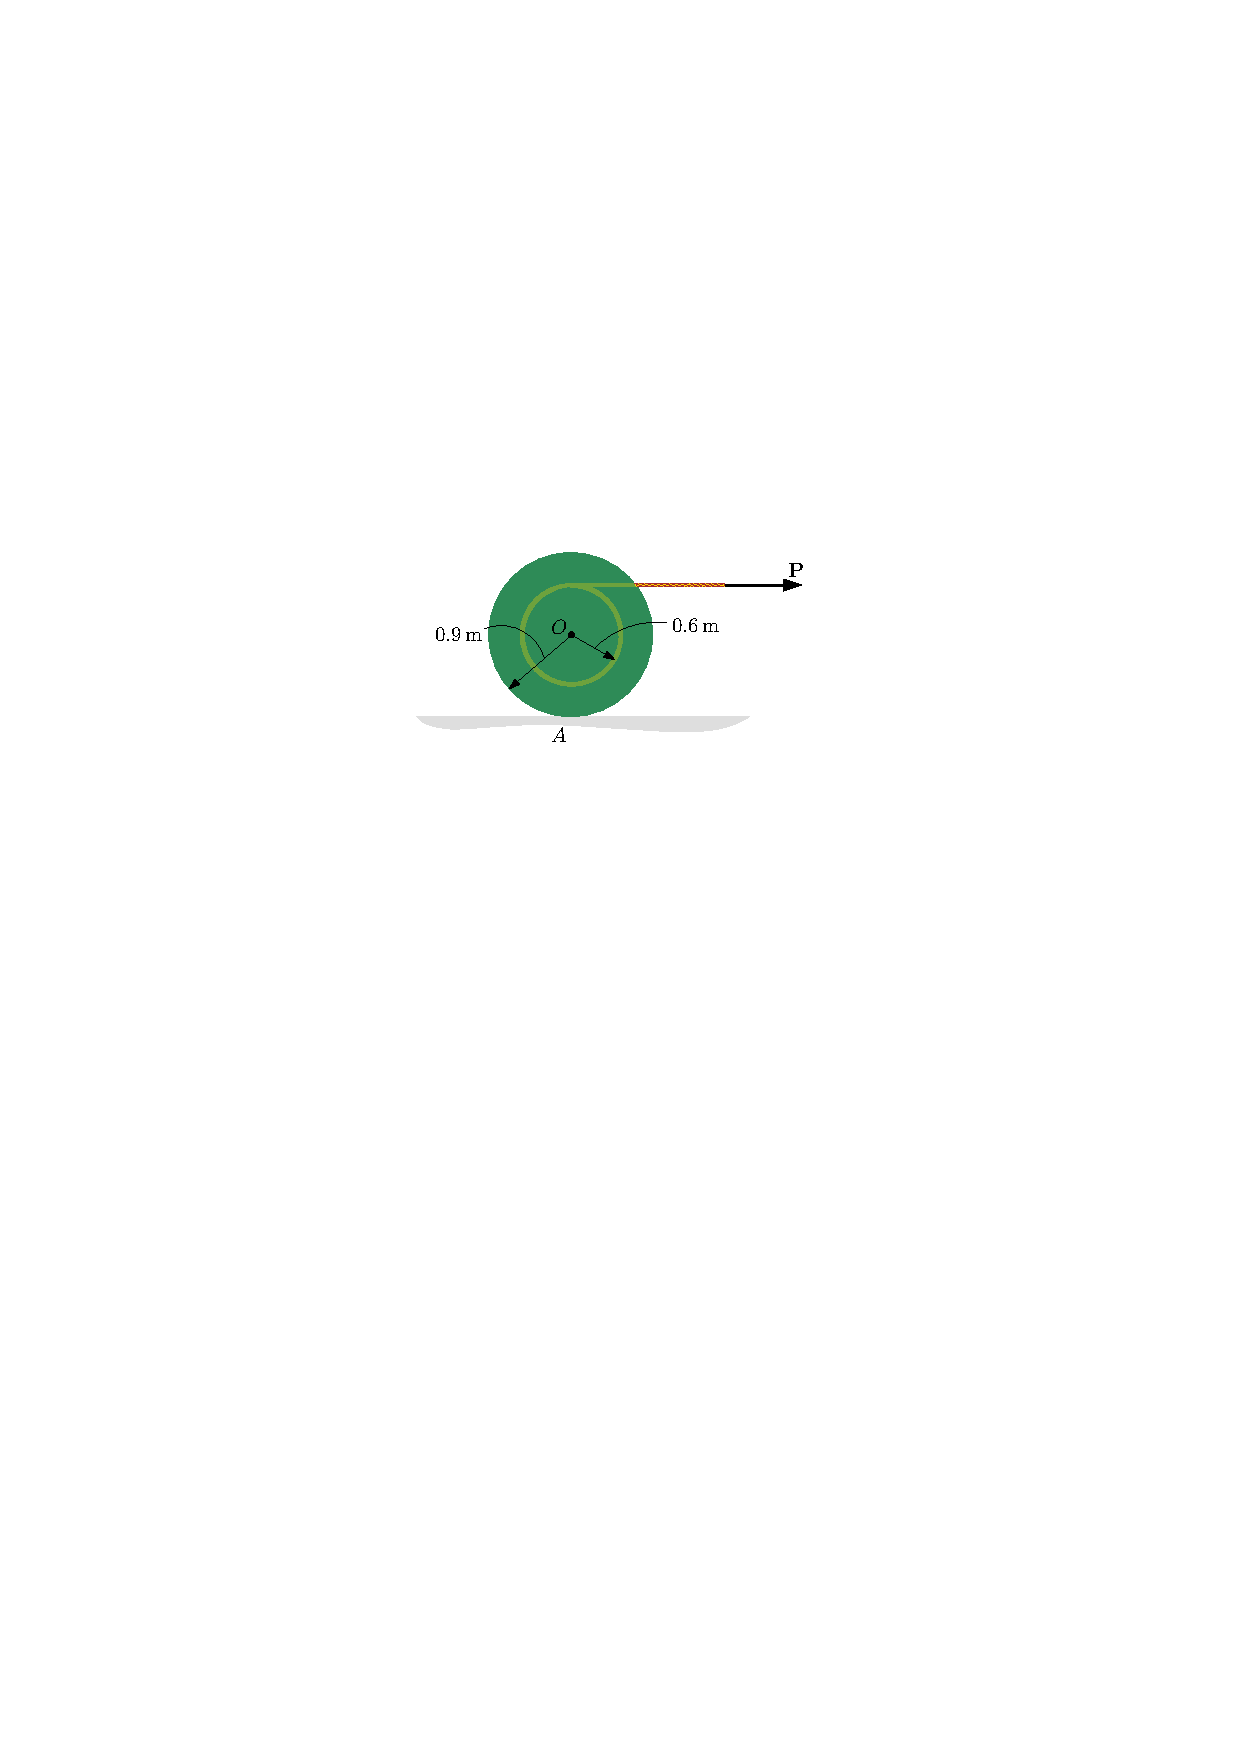
\includegraphics[scale=1.2]{../../images/draw_2_1}
\end{flushright}